\chapter{Literature Review}\label{chap:literature_review}
This chapter provides a comprehensive review of the foundational architectures, innovative compression techniques, and specific models that have significantly contributed to the development of LLMs. By examining these areas, this chapter aims to offer insights into the current state and future directions of natural language processing (NLP) research.

Firstly, an overview of LLMs will be presented based on \cite{naveed2024comprehensive}. This section highlights the rapid evolution of LLMs and the ongoing need for optimization by engineers and researchers. Secondly, previous studies on LLM compression, with a focus on versions of low-rank approximation, will be briefly discussed. The chapter will then introduce the approach of Retrieval-Augmented Generation (RAG) by \cite{lewis2020RAG}, which combines the strengths of pre-trained language models with retrieval mechanisms to enhance performance on knowledge-intensive tasks. Following this, the BART model, which is the focus of this thesis, will be introduced. Finally, the chapter will conclude with a discussion on the evaluation of summarization models using ROUGE metrics.

By providing a detailed examination of these areas, this chapter sets the stage for the subsequent chapters that delve into the practical implementation of a RAG chatbot prototype and the application of low-rank approximation to the BART model.

\section{Overview of LLMs}
The evolution of LLMs can be traced back to earlier models of machine learning that attempted to process and understand language. However, it was the introduction of the Transformer architecture by \cite{vaswani2023attention} that revolutionized the field of NLP, enabling the development of large-scale models capable of capturing complex linguistic patterns and generating coherent text. This architectural innovation laid the foundation for today's models like Google's BERT and OpenAI's GPT series that marked a significant leap in the capabilities of language models. Each iteration of these models has brought improvements in understanding context, generating text, and general language comprehension, culminating in state-of-the-art models that are capable of writing essays, composing poetry, and even generating code.

\cite{naveed2024comprehensive} gives a comprehensive overview of the evolution of LLMs, highlighting the key milestones and breakthroughs that have shaped the landscape of NLP research and applications. The study delves into the architectural advancements, training methodologies, and performance benchmarks of LLMs, providing a detailed account of the progress made in the field over the past decade. By examining the historical context and the latest developments in LLM research, the study offers valuable insights into the current state-of-the-art and the future directions of large-scale language modeling.
\begin{figure}[H]
    \centering
    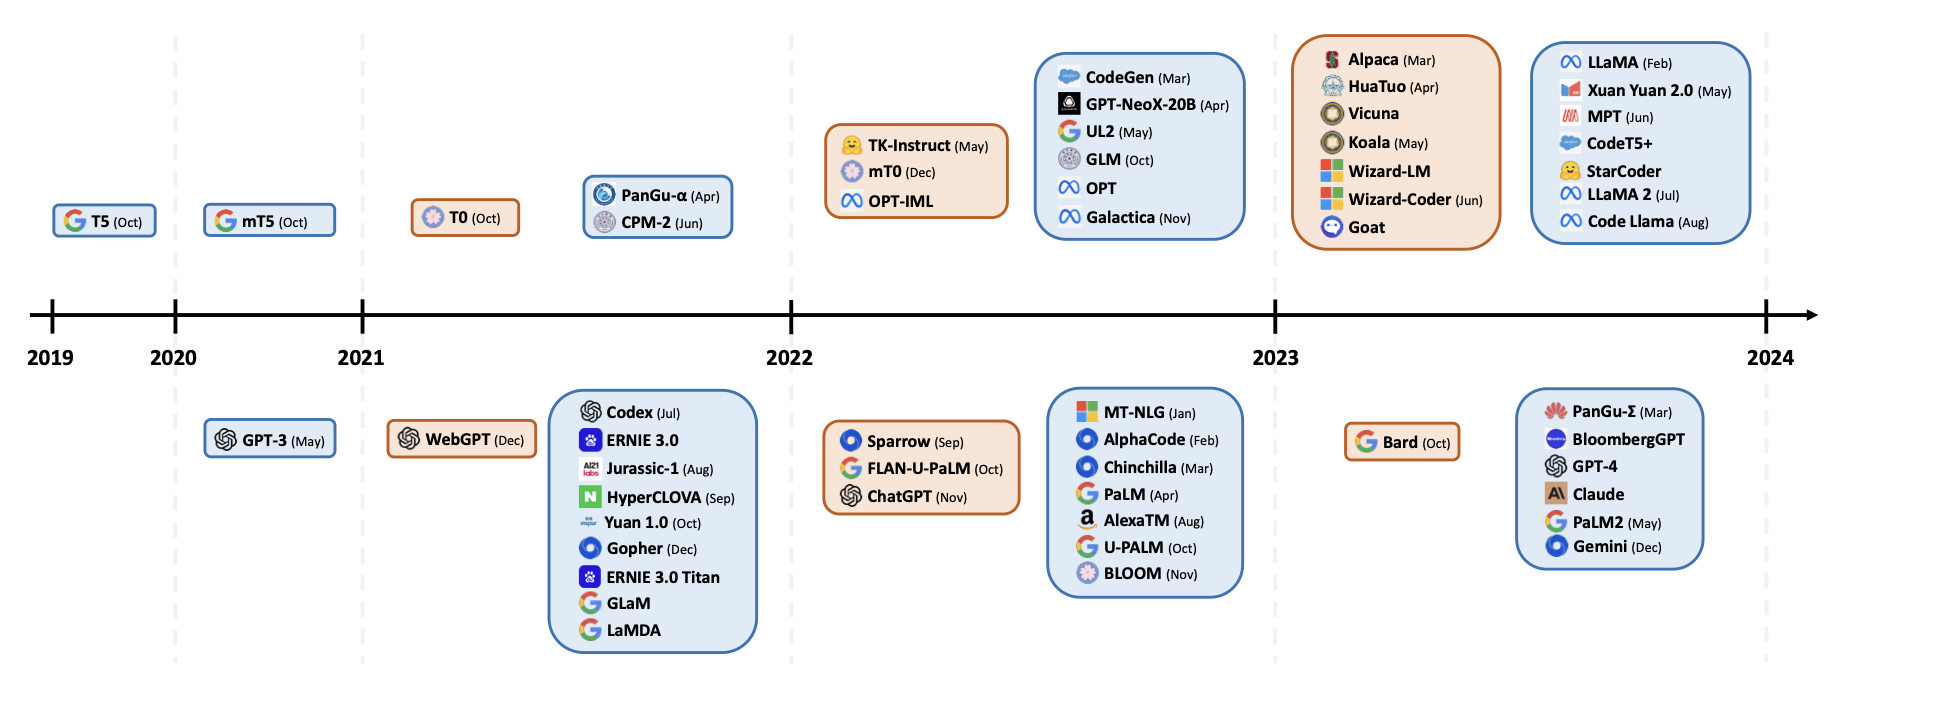
\includegraphics[width=\textwidth]{figs/Chronological_Display.png}
    \caption{Chronological display of LLM releases:  blue cards represent 'pre-trained' models, while orange cards correspond to 'instruction-tuned' models. Models on the upper half signify open-source availability, whereas those on the bottom half are closed-source. - Taken from \cite{naveed2024comprehensive}}
    \label{fig:llm_evolution}
\end{figure}
Figure \ref{fig:llm_evolution} depicts the chronological development of LLM releases, categorizing them based on their nature as either pre-trained or instruction-tuned, and their availability as either open-source or closed-source. This visual representation provides a thorough overview of the diverse models that have emerged over the years, highlighting the rapid advancement and widespread adoption of LLMs in the NLP domain. The chart also reveals a growing trend towards instruction-tuned and open-source models, illustrating the shifting landscape and emerging trends in natural language processing research.

As newer, larger, and more sophisticated models continue to shape the field of NLP, the demand for optimization strategies that enhance the efficiency and performance of these models become increasingly critical. This has spurred a surge in research (also depicted in \cite{naveed2024comprehensive}) focused on model compression, parameter sharing, and other optimization techniques aimed at reducing computational overhead and improving the operational characteristics of LLMs. Through the exploration of innovative methodologies and strategies, researchers are striving to make LLMs more accessible, adaptable, and efficient, thereby unlocking their full potential across a wide range of applications.
This is a product of the increasing demand for LLMs across a vast spectrum of applications, and as the demand grows, so does the need for researchers and developers to understand and thus, by extension, be able to optimize these models to meet the demands of the applications they are used in.

\section{Previous Studies on LLM Compression with Low-Rank Approximation}
    Over the past few year, the increasing demand for LLMs across a vast spectrum of applications, from natural language processing to content generation, has underscored the critical need for optimization strategies tailored to these complex systems. Researchers have delved into a variety of optimization techniques aimed at refining LLMs, with a keen focus on enhancing model efficiency and reducing the computational burden without compromising the specialized performance that these models are known for.
    A key area of investigation has been model compression, which involves reducing the size and complexity of LLMs while maintaining their functionality and performance. \\

        In the realm of LLMs, low-rank approximation has gained substantial traction as a method to fine-tune and streamline models. It has been utilized in various implementations, notably in \cite{hu2021lora} and its subsequent adaptations (\cite{valipour-etal-2023-dylora, zhang2023adaptive, chavan2024oneforall}). These adaptations focus on leveraging low-rank structures to optimize the fine-tuning proces, and in some cases performance of LLMs without extensive resource demands.
        
        Another novel application of this technique is seen in TensorGPT (\cite{xu2023tensorgpt}), which employs a low-rank tensor format to manage large embeddings efficiently. By adopting the Tensor-Train Decomposition (TTD), TensorGPT not only reduces the spatial complexity of LLMs but also potentially boosts their deployment on edge devices. This method treats each token embedding as a Matrix Product State (MPS), enabling the compression of the embedding layer by up to a factor of \(38.40\). Remarkably, this compression is achieved without sacrificing, and in some cases even enhancing, the performance of the model compared to its original configuration.
        
        This focus on low-rank approximation underscores its critical role in advancing the field of LLMs by facilitating more efficient model architectures that maintain high performance while being computationally less demanding.

\section{Retrieval-Augmented Generation}
As LLMs depend on the data they are trained on, they may not always have access to the most up-to-date or specialized information. To address this limitation, \cite{lewis2020RAG} introduced Retrieval-Augmented Generation (RAG), a novel approach that combines the strengths of pre-trained language models (a \emph{generator}), with retrieval mechanisms to enhance performance on knowledge-intensive tasks (\emph{retriever}). RAG models integrate a dense vector index of external knowledge sources, such as Wikipedia, into the generative process, enabling them to access a vast repository of information beyond their pre-training data.
\begin{figure}[H]
    \centering
    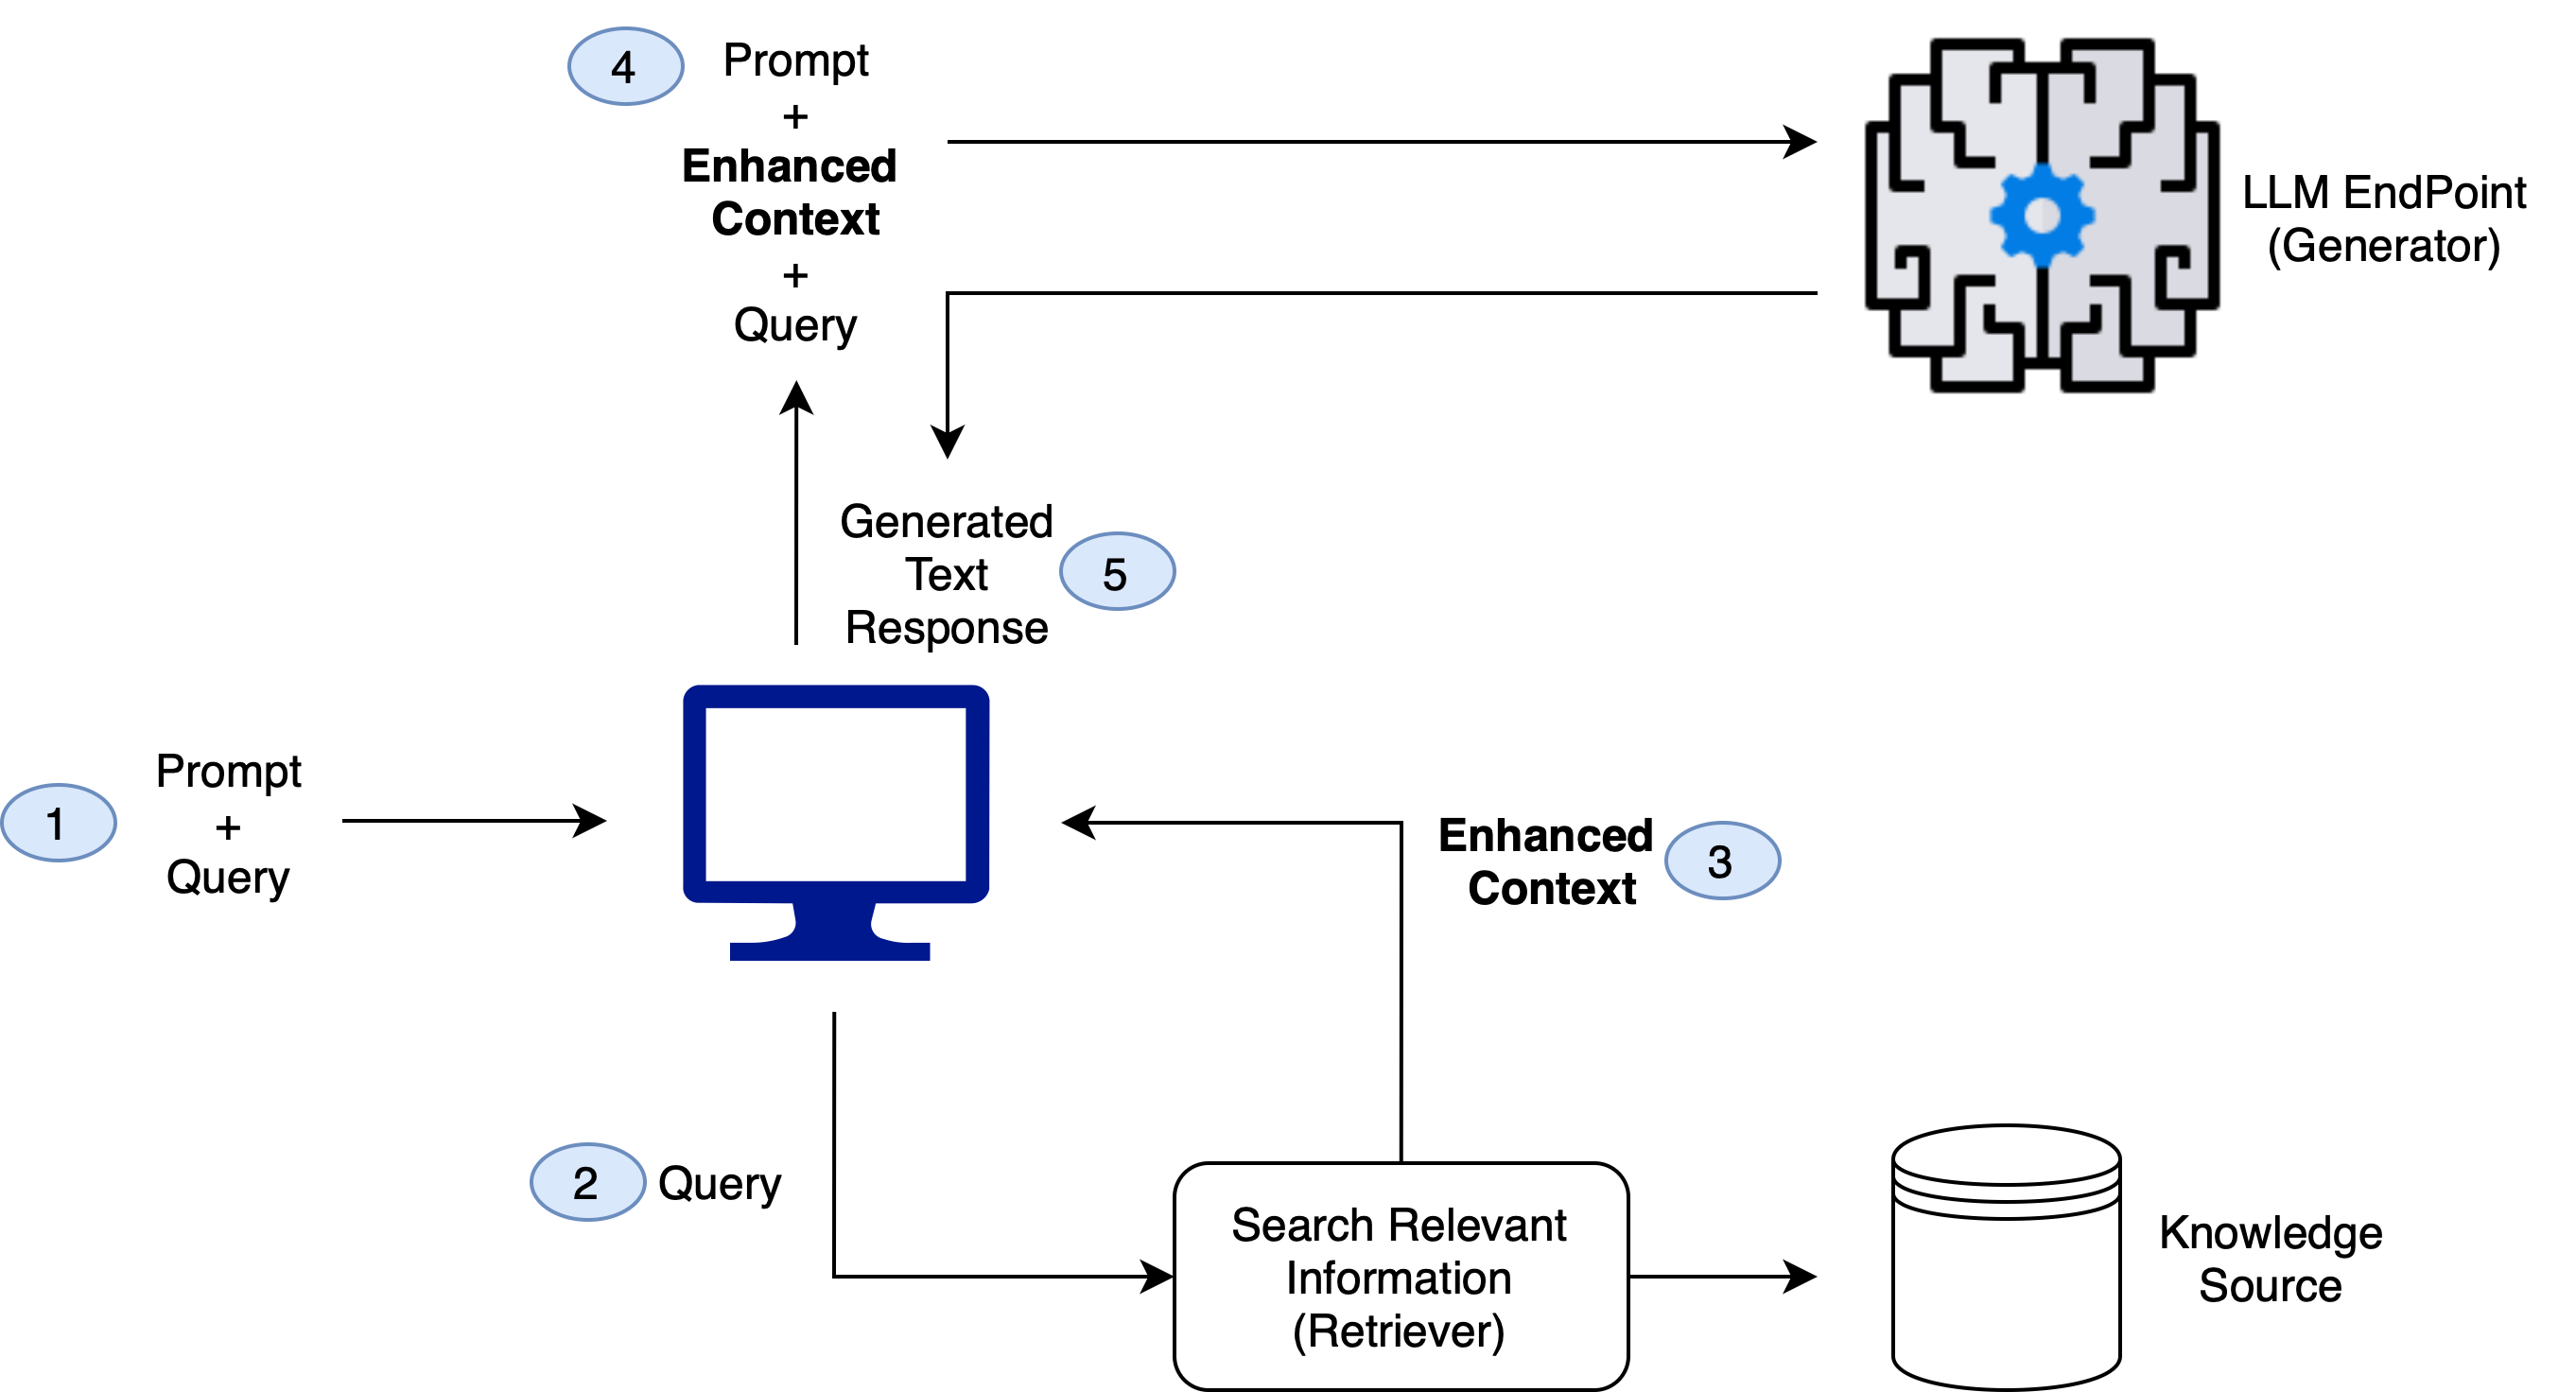
\includegraphics[width=0.8\textwidth]{figs/Flowdiagram.png}
    \caption{Conceptual flow of using RAG with LLMs}
    \label{fig:rag_architecture}
\end{figure}
Figure \ref{fig:rag_architecture} illustrates the conceptual flow of using RAG with LLMs. After prompting a query, the retriever component fetches relevant passages from the external knowledge source based on the input query, which are then used by the generator to produce the final output. This retrieval mechanism enhances the model's ability to generate contextually rich and accurate responses, particularly in knowledge-intensive tasks.
Further benefits of RAG models include:
\begin{itemize}
    \item \textbf{Implementation of Chatbots:} Chatbot applications can benefit from RAG models by providing more accurate and contextually relevant responses to user queries. 
    \item \textbf{Staying up to date with Current Information:} Even if the original training data sources for an LLM are suitable for ones needs, maintaining relevancy is challenging. RAG enables developers to keep generative models up-to-date by incorporating the latest research, statistics, and news. By connecting the LLM directly to live social media feeds, news sites, or other frequently updated information sources, RAG can ensure the model's responses remain current and accurate.
    \item \textbf{Enhanced User Trust:} By providing more accurate and contextually relevant responses, RAG models can enhance user trust in the system. This is particularly important in applications where the information provided must be accurate and up-to-date, such as medical advice, legal consultations, or financial services.
\end{itemize}

\section{The BART Model}\label{sec:bart}
    \textbf{BART: Denoising Sequence-to-Sequence Pre-training for Natural Language Generation, Translation, and Comprehension} by (\cite{lewis2019bart}), introduces BART as a versatile pretraining approach for natural language processing tasks. BART combines the benefits of both autoregressive (like GPT) and autoencoding (like BERT) paradigms into a unified model.

    \subsection{Architecture and Training}
    BART employs a Transformer-based sequence-to-sequence architecture from 
    
    (\cite{vaswani2023attention}), utilizing a bidirectional encoder (similar to BERT) and a left-to-right decoder (similar to GPT) to handle a wide array of tasks from generation to comprehension. For the base model (BART-base) and the large model (BART-large), the encoder and decoder consist of \(6\) and \(12\) layers, respectively (Appendix \ref{appendix:BART}).
    It is trained through a novel denoising objective, where the model reconstructs the original text from corrupted versions. This involves techniques such as token masking (\cite{devlin2019bert}) and text infilling, enhancing the model's ability to understand and generate contextually rich language.
    \begin{figure}[H]
        \centering
        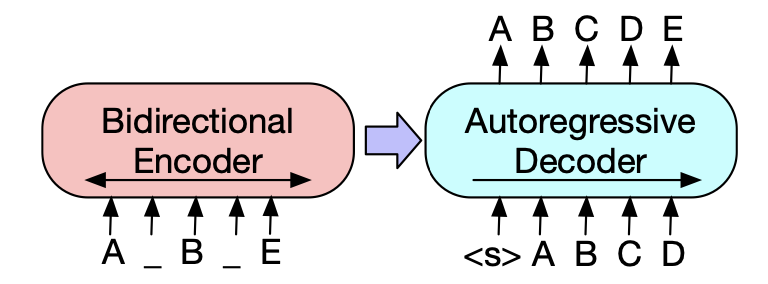
\includegraphics[width=0.8\textwidth]{figs/BART_architecture.png}
        \caption{BART model's processing mechanism - Taken from \cite{lewis2019bart}}
        \label{fig:bart_process}
    \end{figure}
    Figure \ref{fig:bart_process} illustrates the BART model's processing mechanism. The original text sequence [ABCDE] is transformed into a masked version [A[MASK]B[MASK]E]. BART's encoder learns bidirectional representations from this altered input, allowing it to handle inputs that are not aligned with decoder outputs. The decoder then attempts to reconstruct the original sequence autoregressively by optimizing the negative log-likelihood. For fine-tuning, the model processes an uncorrupted document to enhance accuracy and adaptability.
    \subsection{Efficacy and Applications}
    The versatility of BART is demonstrated across various NLP tasks including text generation, comprehension, and translation. Notably, BART outperforms previous work on benchmarks like ROUGE, showcasing substantial improvements particularly in abstractive summarization tasks. The model's ability to fine-tune to specific tasks using pre-trained weights allows it to excel in both generation and comprehension roles, making it a powerful tool for a broad range of applications.

\section{Evaluating Summarization with ROUGE}\label{sec:rouge}
The evaluation of automated summarization models is crucial for assessing their efficiency and effectiveness in capturing the essence of text data. ROUGE (\cite{lin-2004-rouge}), which stands for Recall-Oriented Understudy for Gisting Evaluation, provides a set of metrics that are indispensable for this purpose. Introduced by \cite{lin-2004-rouge}, ROUGE measures compare the overlap between computer-generated summaries and a set of reference summaries typically created by humans.

\paragraph{ROUGE Metrics}
ROUGE includes several specific metrics, such as ROUGE-N (n-gram overlap) and ROUGE-L (longest common subsequence), each suited for different aspects of summarization. For instance, ROUGE-N focuses on the exactness of content at various n-gram levels, providing insights into the precision of the summarization model in replicating key information. In contrast, ROUGE-L assesses the fluency and structure of the generated summaries by measuring sequence similarity, which is crucial for evaluating the narrative flow of the text.

\paragraph{Application and Relevance}
The application of ROUGE in evaluation has been extensively validated across various tasks, including the Document Understanding Conferences (DUC), where it has been used to measure the performance of summarization systems in a competitive environment. These metrics have proven to be reliable indicators of human judgment, making them a standard against which the summarization capabilities of LLMs are benchmarked. The relevance of ROUGE scores lies in their ability to provide quantifiable measures that correlate strongly with human evaluations, thus facilitating the improvement and development of more efficient summarization models.

\paragraph{Significance in LLM Research}
In the context of LLMs, understanding the effectiveness of different compression and optimization techniques often relies on the ability to evaluate how well the reduced models can summarize content. ROUGE metrics serve this purpose by quantifying the trade-offs between model complexity and performance retention, helping researchers and developers optimize LLMs without significant loss in functionality.
